% ------------------------------------------------------------------------
% Trabalho de Conclusão de Curso CEUN-IMT
% ------------------------------------------------------------------------

\title{TCC - Inteligência para transporte público}

\documentclass[
	% -- opções da classe memoir --
	12pt,							% tamanho da fonte
	a4paper,					% tamanho do papel.
	openright,				% capítulos começam em pág ímpar (insere página vazia caso preciso)
	oneside,					% só frente
	%ou twoside,   		% frente e verso
	% -- opções do pacote babel --
	english,					% idioma adicional para hifenização
	brazil						% o último idioma é o principal do documento
	]{abntex2}

%% pacotes utilizados
\usepackage[brazil]{babel}
\usepackage{longtable}
\usepackage{tabularx}
\usepackage{float}
\usepackage[table]{xcolor}
\usepackage[utf8]{inputenc}		% Codificacao do documento (conversão automática dos acentos)
\usepackage[T1]{fontenc}				% Selecao de codigos de fonte.
\usepackage{times}							% Usa a fonte Times
\usepackage{latexsym}
\usepackage{amsmath}
\usepackage{lastpage}						% Usado pela Ficha catalográfica
\usepackage{fancybox}
\usepackage{listings,xcolor}
%Para não definir footnote
\let\footruleskip\undefined
\usepackage{fancyhdr}
\usepackage{lscape}
\usepackage{setspace}
\usepackage{textcomp}						% usar o TM  \texttrademark
\usepackage[pdftex]{graphicx}
\usepackage{subcaption}
\setlength{\belowcaptionskip}{15pt plus 3pt minus 2pt} % Chosen fairly arbitrarily
\usepackage{color}							% Controle das cores
\usepackage{microtype}					% para melhorias de justificação
\usepackage{multirow}
\usepackage{float}
\usepackage{pdfpages}						% incluir outro pdf como anexo
\usepackage{hyperref} 					% controla a formação do índice
\usepackage{booktabs}						% tabelas com linhas variáveis
\usepackage{dirtree}						% árvore de diretórios do apêndice com conteúdo do CD
\usepackage{url}

% Configurações
\def\Ano{\the\year}

\titulo{Inteligência para Transporte Público}
\local{São Caetano do Sul}
\data{\Ano}
\instituicao{Escola de Engenharia Mauá}
\orientador{Tiago Sanches da Silva}
\coorientador{Murilo Zanini de Carvalho}
%{Murilo Zanini de Carvalho}

\tipotrabalho{Trabalho de Conclusão de Curso}
\newcommand{\IMT}{Instituto Mauá de Tecnologia}
\newcommand{\CEUN}{Centro Universitário}
\newcommand{\EscolaCompleto}{\imprimirinstituicao~do~\CEUN~do~\IMT}
\newcommand{\TitutoGraduacao}{Engenheiro de Computação}
\newcommand{\Curso}{Engenharia de Computação}
\newcommand{\DataBanca}{29 de Abril de \Ano}
\newcommand{\Estado}{SP}




% palavras-chave
\newcommand{\PalavraChaveA}{}
\newcommand{\PalavraChaveB}{painel de controle}
\newcommand{\PalavraChaveC}{inteligência artificial}
\newcommand{\PalavraChaveD}{análise de dados}
\newcommand{\PalavraChaveE}{decisão}
\newcommand{\PalavraChaveF}{transporte público}

% key-words
\newcommand{\KeyWordA}{}
\newcommand{\KeyWordB}{dashboard}
\newcommand{\KeyWordC}{artificial intelligence}
\newcommand{\KeyWordD}{data analysis}
\newcommand{\KeyWordE}{decision}
\newcommand{\KeyWordF}{public transportation}

% autores
\newcommand{\FulanoASnome}{Novello}
\newcommand{\FulanoBSnome}{Miraglia}
\newcommand{\FulanoCSnome}{Araujo}
\newcommand{\FulanoDSnome}{}

\newcommand{\AFulano}{\FulanoASnome, Arthur Segura}
\newcommand{\BFulano}{\FulanoBSnome, Luca Ezellner}
\newcommand{\CFulano}{\FulanoCSnome, Lucas Marques}
\newcommand{\DFulano}{}

\newcommand{\FulanoA}{ Arthur Segura Ortiz Novello }
\newcommand{\FulanoB}{ Luca Ezellner Miraglia }
\newcommand{\FulanoC}{ Lucas Marques de Araujo }
\newcommand{\FulanoD}{}

\autor{\FulanoA \\ \FulanoB \\ \FulanoC \\ \FulanoD}




% Banca Examinadora
\newcommand{\Tratamento}[2]{
Prof\ifthenelse{\equal{#2}{m}}{}{$^{\underline{a}}$}.~\ifthenelse{\equal{#1}{Me}}{\ifthenelse{\equal{#2}{m}}{Me.}{Ma.}}{\ifthenelse{\equal{#1}{Esp} \OR \equal{#1}{Dr}}{#1\ifthenelse{\equal{#2}{m}}{. }{$^{\underline{a}}$. }}}
}

%Nome completo dos Examinadores
\newcommand{\ExaminadorA}{Murilo Zanini de Carvalho}
\newcommand{\ExaminadorB}{Sergio Ribeiro Augusto}

%Instituições dos Examinadores
\newcommand{\InstituicaoExaminadorA}{\imprimirinstituicao}
\newcommand{\InstituicaoExaminadorB}{\imprimirinstituicao}

%Título dos Examinadores (Me, Esp ou Dr)
\newcommand{\SexoOrientador}{m}
\newcommand{\SexoCoorientador}{m}
\newcommand{\SexoExaminadorA}{m}
\newcommand{\SexoExaminadorB}{m}

\newcommand{\TituloOrientador}{Me}
\newcommand{\TituloCoorientador}{}
\newcommand{\TituloExaminadorA}{Me}
\newcommand{\TituloExaminadorB}{Dr}

\newcommand{\TratamentoOrientador}  {\Tratamento{\TituloOrientador}{\SexoOrientador}}
\newcommand{\TratamentoCoorientador}{\Tratamento{\TituloCoorientador}{\SexoCoorientador}}
\newcommand{\TratamentoExaminadorA} {\Tratamento{\TituloExaminadorA}{\SexoExaminadorA}}
\newcommand{\TratamentoExaminadorB} {\Tratamento{\TituloExaminadorB}{\SexoExaminadorB}}

% alterando valores do ABNTEX2
\renewcommand{\orientadorname}{\ifthenelse{\equal{\SexoOrientador}{m}}{Orientador}{Orientadora}}
\renewcommand{\coorientadorname}{\ifthenelse{\equal{\SexoCoorientador}{m}}{Coorientador}{Coorientadora}}





% Informações de dados para FOLHA DE ROSTO e FOLHA DE APROVAÇÃO
\preambulo{\imprimirtipotrabalho~apresentado à~\EscolaCompleto~como requisito parcial para a obtenção de título de~\TitutoGraduacao. \newline Área de Concentração:~\Curso}

\newcommand{\preambuloaprovado}{\imprimirtipotrabalho~aprovado como requisito parcial para a obtenção de título de~\TitutoGraduacao~pela \EscolaCompleto. \newline Área de Concentração:~\Curso}





%Ficha Catalográfica
%CDU - Classificação Decimal Universal
%6 - Ciências Aplicadas. Medicina. Tecnologia.
%2 - Engenharia. Tecnologia geral.
%1 - Engenharia mecânica em geral. Tecnologia nuclear. Engenharia elétrica. Maquinaria
%3 - Engenharia elétrica
\newcommand{\CDU}{CDU 621.398}
\newcommand{\Cutter}{T272}





% tamanho da fonte das seções
\renewcommand{\ABNTEXchapterfontsize}{\normalsize}
\renewcommand{\ABNTEXsectionfontsize}{\normalsize}
\renewcommand{\ABNTEXsubsectionfontsize}{\normalsize}
\renewcommand{\ABNTEXsubsubsectionfontsize}{\normalsize}
\renewcommand{\ABNTEXsubsubsubsectionfontsize}{\normalsize}
% tipo da fonte das seções
\renewcommand{\ABNTEXchapterfont}{\normalfont\bfseries}
\renewcommand{\ABNTEXsectionfont}{\normalfont\bfseries}
\renewcommand{\ABNTEXsubsectionfont}{\normalfont\bfseries}
\renewcommand{\ABNTEXsubsubsectionfont}{\normalfont\bfseries}
\renewcommand{\ABNTEXsubsubsubsectionfont}{\normalfont\bfseries}
\renewcommand{\legend}{\ABNTEXfontereduzida\centering}

% Espaçamentos 
% Margens
\setlrmarginsandblock{3cm}{2cm}{*}
\setulmarginsandblock{3cm}{2cm}{*}
\checkandfixthelayout
\setlength\afterchapskip{\onelineskip}
\setlength{\parindent}{0 mm} % recuo




% Criando Quadros
\newcounter{quadroCount}
\setcounter{quadroCount}{0}
\newenvironment{quadro}[2] % #1 caption e #2 label
{% This is the begin code
  \refstepcounter{quadroCount}
  \centering
  {Quadro} \arabic{quadroCount}: #2\\ 
	\label{#1}
}
{% This is the end code
}

% Bibliografia
\usepackage[brazilian,hyperpageref]{backref}		% Paginas com as citações na bibl
\usepackage[
  alf,
	abnt-emphasize=bf,
	abnt-url-package=hyperref,
	abnt-etal-list=0, % 6023 - mostra todos os nomes nas referências
	abnt-etal-cite=3, % 10520 - número de autores antes de ser et al
	recuo=0.0cm %0.5cm
]{abntex2cite}										% Citações padrão ABNT


% Configurações o PDF
\makeatletter
	\hypersetup{
	pdftitle={\imprimirtitulo},
	pdfauthor={{\imprimirautor~e~\imprimirorientador}},
	pdfsubject={\imprimirpreambulo},
	pdfkeywords={\PalavraChaveA\\}{\PalavraChaveB\\}{\PalavraChaveC\\}{\PalavraChaveD\\}{\PalavraChaveE},
	colorlinks=true,						% não desenha o retângulo em referências
	linkcolor=black, 						% cor das referências cruzadas
	citecolor=black, 						% cor das citações - 10520
	filecolor=black, 						% cor dos arquivos
	urlcolor=black, 						% cor dos sites
	bookmarksdepth=4
}
\makeatother



% Início do documento
\begin{document}
	\lstset{
		string=[s]{"}{"},
		stringstyle=\color{red},
		comment=[l]{:},
		commentstyle=\color{black},
		basicstyle=\tiny,
		% backgroundcolor=\color{lightgray},
	}

		% Elementos pré-textuais
    \pretextual
		\renewcommand{\imprimircapa}{%
	\begin{capa}%
		\center
		\textbf{\imprimirautor}

		\vspace*{\fill}

		\textbf{\imprimirtitulo}

		\vspace*{\fill}
		    
		{\imprimirlocal}
		\par
		{\imprimirdata}
	\end{capa}
}
\imprimircapa
		\makeatletter
\renewcommand{\folhaderostocontent}{
	\begin{center}
		{\ABNTEXchapterfont \textbf{\imprimirautor}}

		\vspace*{\fill}\vspace*{\fill}

		\ABNTEXchapterfont \textbf{\imprimirtitulo}

		\vspace*{\fill}
		
		\normalfont

		\begin{flushright}
			\abntex@ifnotempty{\imprimirpreambulo}{
				\hspace{.45\textwidth}
	
				\begin{minipage}{.55\textwidth}
					\SingleSpacing
					\imprimirpreambulo
					
					\vspace*{.7cm}

					{\imprimirorientadorRotulo~\imprimirorientador\par}
					\abntex@ifnotempty{\imprimircoorientador}{
						{\imprimircoorientadorRotulo~\imprimircoorientador}
					}
				\end{minipage}
	
				\vspace*{\fill}
			}
		\end{flushright}

		\vspace*{\fill}

		{\imprimirlocal}
		\par
		{\imprimirdata}
	\end{center}
}
\makeatother

\imprimirfolhaderosto*
%


% deixar essas duas linhas de espaço!!!!
		\begin{fichacatalografica}
	%\includepdf{Ficha_catalografica.pdf}
% ou

\newcolumntype{L}[1]{>{\raggedright\let\newline\\\arraybackslash\hspace{0pt}}p{#1}}
\newcounter{cont}
\setcounter{cont}{1}

\newif\ifnAlunosTresMais
\ifthenelse{\equal{\FulanoDSnome}{}}{\nAlunosTresMaisfalse}{\nAlunosTresMaistrue}

%\newif\ifnAlunosTresMais
%\ifthenelse{\equal{\FulanoDSnome}{}}{\nAlunosTresMaisfalse}{\nAlunosTresMaistrue}

\vspace*{\fill}
\ifnAlunosTresMais
	\begin{table}[!b]
  		\setlength{\arrayrulewidth}{0.75pt}
		\begin{tabular}{|L{1cm}L{11.5cm}|}
			\hline
			~ & ~ \\
			{\fontsize{9pt}{9pt}\selectfont \Cutter} & 
			{\fontsize{9pt}{9pt}\selectfont \hspace{0.37cm}
			\imprimirtitulo\ / \FulanoA...[et al.] - \local {} : CEUN-IMT, \imprimirdata.}\\
			~ & \hspace{0.37cm}
			{\fontsize{9pt}{9pt}\selectfont \pageref{LastPage} p.}\\
			~ & ~ \\
			~ & \hspace{0.37cm}
			{\fontsize{9pt}{1cm}\selectfont \imprimirtipotrabalho~- \EscolaCompleto, \local,~\Estado,~\imprimirdata.}\\
			~ & ~ \\
			~ & ~ \\
			~ & \hspace{0.37cm}
			{\fontsize{9pt}{1cm}\selectfont \imprimirorientadorRotulo:~\imprimirorientador}\\	
			~ & ~ \\
			~ & \hspace{0.37cm}
			{\fontsize{9pt}{1cm}\selectfont 
			\ifthenelse{\equal{\PalavraChaveA}{}}{}{1. \PalavraChaveA} 
			\ifthenelse{\equal{\PalavraChaveB}{}}{}{2. \PalavraChaveB} 
			\ifthenelse{\equal{\PalavraChaveC}{}}{}{3. \PalavraChaveC} 
			\ifthenelse{\equal{\PalavraChaveD}{}}{}{4. \PalavraChaveD} 
			\ifthenelse{\equal{\PalavraChaveE}{}}{}{5. \PalavraChaveE} 
     	\ifthenelse{\equal{\FulanoASnome}{}}{}{\Roman{cont}. \AFulano.\setcounter{cont}{\value{cont}+1}} 
     	\ifthenelse{\equal{\FulanoBSnome}{}}{}{\Roman{cont}. \BFulano.\setcounter{cont}{\value{cont}+1}} 
     	\ifthenelse{\equal{\FulanoCSnome}{}}{}{\Roman{cont}. \CFulano.\setcounter{cont}{\value{cont}+1}} 
     	\ifthenelse{\equal{\FulanoDSnome}{}}{}{\Roman{cont}. \DFulano.\setcounter{cont}{\value{cont}+1}} 
     	\Roman{cont}. \IMT. \CEUN. \imprimirinstituicao. \setcounter{cont}{\value{cont}+1}
     	\Roman{cont}. Tí­tulo.}	\\
			~ & ~ \\
			~ & \hspace{9cm}
			{\fontsize{9pt}{1cm}\selectfont \CDU} \\
 	 		\hline
  		\end{tabular}
	\end{table}
\else
	\begin{table}[!b]
	\centering
  		\setlength{\arrayrulewidth}{0.75pt}
		\begin{tabular}{|L{1cm}L{11.5cm}|}
			\hline
			~ & ~ \\
% 			{\fontsize{9pt}{9pt}\selectfont \Cutter} 
            & 
			{\fontsize{9pt}{9pt}\selectfont \AFulano}\\
			~ & {\fontsize{9pt}{9pt}\selectfont \hspace{0.37cm}
			\imprimirtitulo\ / \ifthenelse{\equal{\FulanoASnome}{}}{}{\FulanoA}\ifthenelse{\equal{\FulanoBSnome}{}}{}{, \FulanoB}\ifthenelse{\equal{\FulanoCSnome}{}}{}{, \FulanoC}. - \imprimirlocal: CEUN-IMT, \imprimirdata.}\\
			~ & {\fontsize{9pt}{9pt}\selectfont \hspace{0.37cm} \pageref{LastPage} p.}\\
			~ & ~ \\
			~ & \hspace{0.37cm}
			{\fontsize{9pt}{1cm}\selectfont \imprimirtipotrabalho~-~\EscolaCompleto, \imprimirlocal, \Estado, \imprimirdata.}\\
			~ & ~ \\
			~ & ~ \\
			~ & \hspace{0.37cm}
			{\fontsize{9pt}{1cm}\selectfont \imprimirorientadorRotulo:~Prof. Me.~\imprimirorientador}\\	
			~ & ~ \\
			~ & \hspace{0.37cm}
			{\fontsize{9pt}{1cm}\selectfont 
			\ifthenelse{\equal{\PalavraChaveA}{}}{}{1. \PalavraChaveA}. 
			\ifthenelse{\equal{\PalavraChaveB}{}}{}{2. \PalavraChaveB}. 
			\ifthenelse{\equal{\PalavraChaveC}{}}{}{3. \PalavraChaveC}. 
			\ifthenelse{\equal{\PalavraChaveD}{}}{}{4. \PalavraChaveD}. 
     	\ifthenelse{\equal{\FulanoBSnome}{}}{}{\Roman{cont}. \BFulano.\setcounter{cont}{\value{cont}+1}} 
     	\ifthenelse{\equal{\FulanoCSnome}{}}{}{\Roman{cont}. \CFulano.\setcounter{cont}{\value{cont}+1}} 
     	\Roman{cont}. \IMT. \imprimirinstituicao. \setcounter{cont}{\value{cont}+1}
     	\Roman{cont}. Tí­tulo.}	\\
			~ & ~ \\
% 			~ & \hspace{9cm}
% 			{\fontsize{9pt}{1cm}\selectfont \CDU} \\			
 	 		\hline
  		\end{tabular}
	\end{table}
\fi

\end{fichacatalografica}

		\makeatletter
\begin{folhadeaprovacao}
	\begin{center}
		{\ABNTEXchapterfont \textbf{\imprimirautor}}
		
		\vspace*{\fill}\vspace*{\fill}
		
		\begin{center}
			\ABNTEXchapterfont \textbf{\imprimirtitulo}
		\end{center}

		\vspace*{\fill}
		\hspace{.45\textwidth}

		\normalfont

		\begin{flushright}
			\begin{minipage}{.55\textwidth}
				\preambuloaprovado
			\end{minipage}%
		\end{flushright}

		\vspace*{\fill}
	\end{center}
		
	\normalfont

	Banca examinadora:

	\begin{center}
		\TratamentoOrientador~\imprimirorientador \\ \imprimirorientadorRotulo \\
		\vspace*{\fill}
		\abntex@ifnotempty{\imprimircoorientador}{
			\TratamentoCoorientador~\imprimircoorientador \\ \imprimircoorientadorRotulo \\ \imprimirinstituicao\\
			\vspace*{\fill}
		}
		\TratamentoExaminadorA~\ExaminadorA \\ Avaliador\\
		\vspace*{\fill}
		\TratamentoExaminadorB~\ExaminadorB \\ Avaliador\\
		\vspace*{\fill}
	\end{center}
	
	\begin{center}
		\vspace*{0.5cm}

		{\imprimirlocal}, \DataBanca.
	\end{center}
\end{folhadeaprovacao}
\makeatother

		\begin{dedicatoria}
    \vspace*{\fill}
	\begin{flushright}
		\textit{Aos nossos pais, irmãos e irmãs, amigos e colegas de formação.}
	\end{flushright}
\end{dedicatoria}

		\begin{agradecimentos}
XXXXX
\\\\
XXXXX
\\\\
XXXXX
\\\\
XXXXX
\\\\
XXXXX
\end{agradecimentos}

		\begin{epigrafe}
    \vspace*{\fill}
	\begin{flushright}
		\textit{``XX''} \\("XX")\\
	\textit{\bfseries XX}
	\end{flushright}
\end{epigrafe}

		\begin{resumo}
\indent
\par O projeto em questão tem como objetivo a criação de um dashboard que monitora as demandas das   frotas   de veículos, no caso as linhas de ônibus da SPTrans, empresa responsável pelos ônibus da cidade de São Paulo. Para esse monitoramento, serão utilizados dados públicos fornecidos pela SPTrans, como rotas dos ônibus, dados de GPS, linhas e paradas, por exemplo, que serão enriquecidos com outras informações, como datas e locais de eventos, situação das linhas de trens e metrôs, informações meteorológicas e o trânsito na cidade.
\par Com posse dessas informações, o projeto também visa o desenvolvimento de um modelo de inteligência artificial que poderá ser utilizado pela equipe operacional da SPTrans para auxiliar o controle de demanda das frotas, indicando se são necessários mais ou menos ônibus em cada linha. Os dados apresentados pelo modelo também poderão ser utilizados por cidadãos comuns que procuram uma maior transparência para observar a situação das linhas e potenciais fatores que poderão alterar o fluxo normal do transporte público.
\par Considerando que atualmente muitos dados do transporte coletivo são públicos, mas não existe uma plataforma centralizadora dessas informações que seja capaz de auxiliar as pessoas no que diz respeito a uma visão geral das condições das linhas de ônibus, o presente trabalho pretende contribuir positivamente para melhorar a experiência dos usuários e trazer uma visão mais transparente do serviço como um todo.
\par Para a construção do sistema foram utilizadas ferramentas como Python, Django, Django-REST, Celery e Amazon Web Services (AWS), que possibilitaram o desenvolvimento do dashboard e todas suas funcionalidades, desde a aquisição de dados externos, até a manipulação desses dados e implantação da plataforma na nuvem.
    
\textbf{Palavras-chaves}: \PalavraChaveA.~\ifthenelse{\equal{\PalavraChaveB}{}}{}{\PalavraChaveB.~}\ifthenelse{\equal{\PalavraChaveC}{}}{}{\PalavraChaveC.~}\ifthenelse{\equal{\PalavraChaveD}{}}{}{\PalavraChaveD.~}\ifthenelse{\equal{\PalavraChaveE}{}}{}{\PalavraChaveE.~}\ifthenelse{\equal{\PalavraChaveF}{}}{}{\PalavraChaveF.~}

\end{resumo}

		\begin{resumo}[Abstract]
	\begin{otherlanguage*}{english}
	\indent
	\par This project aims to create a dashboard that monitors the demand of vehicles in bus lines of SPTrans, the company responsible for buses in the city of São Paulo. For this monitoring, public data provided by SPTrans was used, such as bus routes, GPS data, lines and stops, for example, which will be enriched with other information, like dates and locations of events, status of train and subway lines, weather information and traffic around the city.
	\par Although a lot of public transport data is public available, there isn’t a system to aggregate all this information that would be able to help people who use this kind of transport on a daily basis with a overview about the lines condition. The present work intends to contribute positively to improve the user experience and bring a more transparent and complete view of the service.
	\par During the development, tools such as Python, Django, Django-REST, Celery and Amazon Web Services (AWS) were used, which made it possible to create a dashboard and all its features, from the acquisition of external data, to the manipulation of that data and deployment of the platform in a cloud platform.
	\\
	\\
	\textbf{Key-words}: ~\ifthenelse{\equal{\KeyWordB}{}}{}{\KeyWordB.~}\ifthenelse{\equal{\KeyWordC}{}}{}{\KeyWordC.~}\ifthenelse{\equal{\KeyWordD}{}}{}{\KeyWordD.~}\ifthenelse{\equal{\KeyWordE}{}}{}{\KeyWordE.~}\ifthenelse{\equal{\KeyWordF}{}}{}{\KeyWordF.~}
	\end{otherlanguage*}
\end{resumo}

		\listoffigures*
			\cleardoublepage
		\listoftables*
			\cleardoublepage
		\begin{siglas}
%    \item[AUROC] \textit{Area Under ROC}
    \item[API] \textit{Application Programming Interface}
%    \item[ASM] \textit{Active Shape Model}
%    \item[AutoML] \textit{Automatic Machine Learning}
%    \item[BBC] \textit{British Broadcasting Corporation}
%    \item[CNTK] \textit{Microsoft Cognitive Toolkit}
%    \item[CPU] \textit{Central Processing Unit}
%    \item[CRISP-DM] \textit{Cross Industry Standard Process for Data Mining}
%    \item[CUDA] \textit{Compute Unified Device Architecture}
%    \item[cuDNN] \textit{CUDA Deep Neural Network}
%    \item[FBFFT] \textit{Facebook authored Fast Fourier Transform}
%	\item[FFT] \textit{Fast Fourier Transform}
%	\item[FPS] \textit{Frames Per Second}
%	\item[FSF] \textit{Free Software Foundation}
%	\item[GPU] \textit{Graphics Processing Unit}
%	\item[HOG] \textit{Histograms of Oriented Gradients}
%	\item[IaaS] \textit{Infrastructure as a Service}
	\item[CPTM] {Companhia Paulista de Trens Metropolitanos}
	\item[IBGE] {Instituto Brasileiro de Geografia e Estatística}
	\item[IA]  {Inteligência Artificial}
%   \item[SA-Trans] {Santo André Transportes}
	\item[SP-Trans] {São Paulo Transportes}
	\item[AWS] \textit{Amazon Web Services}
	\item[EC2] \textit{Elastic Compute Cloud}
	\item[SQS] \textit{Simple Queue Service}
	\item[CRUD] \textit{Create, Read, Update, Delete}
	\item[REST] \textit{Representational State Transfer}
%	\item[IP] \textit{Internet Protocol}
%	\item[IT] \textit{Information Tecnology}
%	\item[JS] \textit{Javascript}
%	\item[LGBM] \textit{Light Gradient Boosting Machine}
%	\item[OMS] {Organização Mundial da Saúde}
	\item[OpenCV] \textit{Open Source Computer Vision}
%	\item[OpenGL] \textit{Open Graphics Library}
%	\item[PaaS] \textit{Platform as a Service}
%	\item[PCA] \textit{Principal Component Analysis}
%	\item[PERS] \textit{Personal Emergency Response Systems}
%	\item[R-CNN] \textit{Region-based Convolutional Neural Network}
%	\item[RAM] \textit{Random Access Memory}
%	\item[ROC] \textit{Receiver Operating Characteristics}
%	\item[SaaS] \textit{Software as a Service}
%	\item[SNARC] \textit{Stochastic Neural Analog Reinforcement Computer}
%	\item[SVM] \textit{Support Vector Machine}
%	\item[TFX] \textit{TensorFlow Extended}
%	\item[TPU] \textit{Tensor Processing Unit}
%	\item[WebGL] \textit{Web Graphics Library}
	\item[YOLO] \textit{You Only Look Once}
\end{siglas}

		\begin{simbolos}
%  \item[$ \Omega $] Impedância
%  \item[$ V $] Tensão
%  \item[$ T $] Tesla
%  \item[$ B $] Campo Magnético
%  \item[$ bps $] bits por segundo
%  \item[$ Bps $] Bytes por segundo
%  \item[$ Hz $] Frequência 
%  \item[$ degrees/s $] Velocidade angular em graus por segundo
\end{simbolos}

		\pdfbookmark[0]{\contentsname}{toc}
		\tableofcontents*
			\cleardoublepage

		% Elementos textuais
		\textual
		\setlength{\parindent}{7ex}
		\setlength{\parskip}{1em}
		%\setlength{\baselineskip}{1.5cm}
		\chapter{Introdução}
\label{Cap:Intro}

% Capítulo 1: Introdução

\section{Transporte público}
\indent
\par O transporte público caracteriza-se como uma opção amplamente utilizada por pessoas a fim de garantirem suas necessidades de locomoção. Por possuir um preço mais acessível e muitas vezes ser mais rápido e prático, 65\% da população das capitais do Brasil utiliza essa forma de transporte, como aponta um estudo realizado pelo Instituto de Pesquisa Econômica Aplicada (Ipea) \cite{Peduzzi2011}.
\par Foi direcionado o valor de R\$ 707 milhões no ano de 2019 pela União para a área de mobilidade urbana e trânsito, como indica a Lei Orçamentária Anual (LOA n° 13.808/2019). Desse montante, especificamente para o transporte público coletivo, foram separados apenas R\$ 348 milhões, uma fatia de 0,01\% do orçamento total da União \cite{NTUrbano}.
\par De acordo com uma estimativa do BNDES, em 2015, seria necessário investir mais de R\$ 234 bilhões em transporte público para resolver os problemas da área nas principais regiões metropolitanas do país, portanto, caso mantido o nível de investimento atual, levaria mais de 600 anos para atingir o montante proposto pelo BNDES \cite{Santos2015}. Tendo em vista o baixo investimento frente a demanda, é esperado que o transporte público gere um elevado nível de insatisfação em seus usuários, o que o IPEA demonstrou em outra pesquisa realizada em 2011 e 2012, na qual o transporte público foi avaliado por mais de 60\% do público como "péssimo ou ruim"  \cite{Santos2015}.
\par Para entender a situação em que se encontra o transporte, o primeiro passo é olhar como o país se urbanizou. No último século, o Brasil passou por um intenso processo de industrialização, o que gerou um forte êxodo rural e principalmente uma migração da população do Nordeste para o Sul e Sudeste, onde se concentrou a produção industrial do país.
\par Esse crescimento populacional nas metrópoles foi acompanhado por uma grande valorização dos terrenos e moradias nas áreas centrais das cidades. Com isso é observado um efeito de gentrificação, afastando a classe trabalhadora para regiões mais periféricas, longe de onde se concentra a maior parte da oferta de emprego, o que gerou uma demanda por transporte, crescente até os dias atuais.
Tendo em vista esse cenário, a população começou a consumir cada vez mais carros populares, que contam com incentivo do governo para serem produzidos. Com isso, o que se vê nos ambientes urbanos são ruas congestionadas e ônibus lotados \cite{PenaSD}.

\section{Justificativa}
\indent
\par O presente trabalho tem por motivação a grande quantidade de cidadãos de São Paulo que apresentam adversidades quando se trata da utilização dos ônibus da cidade, como o elevado tempo de espera e as altas taxas de ocupação interna, que lideram as reclamações do Reclame Aqui \cite{ReclameAqui1} \cite{ReclameAqui2}. Além disso, a criação de um processo inteligente e automatizado que auxilie os gestores da SPTrans (empresa responsável pelo gerenciamento dos transportes do município de São Paulo) no ajuste das frotas de ônibus justificam esse projeto.
\par Ainda olhando para o transporte público de São Paulo, hoje o sistema todo, composto de ônibus, trens, metrô e outros modais, transporta mais de 17 milhões de passageiros diariamente na capital \cite{G1SaoPaulo}, sendo que dessa quantidade, 7 milhões utilizam as linhas de ônibus da cidade, que hoje conta com mais de 1.300 linhas \cite{MobilidadeSampa}, sendo as principais a Terminal Bandeira / Terminal Varginha, Terminal Jardim  ngela / Metrô Santa Cruz e Hospital Itaim / Guaianazes , que juntas transportam cerca de 100 mil passageiros por dia \cite{Viatrolebus}.
\par Hoje, a SPTrans disponibiliza uma API, atualizada em tempo real, com informações de localização dos veículos, velocidades, pontos de parada e quantidade de ônibus ativos. Apesar de provavelmente a empresa contar com uma solução proprietária, decidimos coletar essas informações e enriquece-las com outros dados disponíveis para desenvolver o nosso trabalho.

\section{Objetivos}
\indent
\par Tendo em vista o cenário apresentado, pretende-se criar um \textit{dashboard} para centralizar informações e agilizar a tomada de decisão. Tendo como base dados coletados durante os trajetos de ônibus, informações extraídas de APIs públicas,  a ferramenta irá apoiar os gestores da SPTrans no controle do fluxo de tráfego, além de ser um ótimo indicador para a população que deseja ter uma visão geral do transporte público de São Paulo. 
\par Além disso, o \textit{dashboard} será atualizado em tempo real, exibindo gráficos e indicadores de maneira sucinta, com a possibilidade de aplicação de filtros nas consultas. Considerando o volume de passageiros para um determinado dia e horário somados a dados externos, a ferramenta permitirá (em trabalhos futuros) utilizar algoritmos de inteligência artificial para identificar padrões históricos e prever futuras demandas nas frotas de ônibus, facilitando o controle do serviço e auxiliando no dia a dia do transporte urbano na cidade.

\section{Contribuições do trabalho}
\indent
\par Este trabalho tem como contribuição a melhoria na tomada de decisões da administradora de ônibus (SPTrans) onde será possível, de forma centralizada, a visualização de dados e gráficos por meio de um \textit{dashboard}. Além disso, pode-se citar como contribuição a diminuição do tempo de espera e ocupação dos transportes, resultando em uma melhor qualidade de vida para a população de São Paulo.

\section{Questão central da pesquisa e seus impactos}
\indent
\par Os benefícios esperados com esse trabalho de conclusão de curso são proporcionar uma melhor qualidade locomotiva dos ônibus de São Paulo e proporcionar uma melhor gestão aos envolvidos da SPTrans, otimizando e inovando a forma de ver os dados. O transporte público, mais especificamente, os ônibus, podem causar estresse. A sensação pode estar relacionada a fatores como as condições do transporte, o desconforto de estar entre muitas pessoas e o elevado tempo de espera.
\par Com a visualização dos dados disponíveis os gestores e responsáveis poderão ver a situação de lotação e do tempo de espera através do \textit{dashboard}. Numa situação crítica, eles poderão solicitar um aumento da frota e reduzir o desconforto de andar em um veículo com excesso de pessoas além de reduzir o tempo de espera. Essas ações impactam diretamente na saúde das pessoas reduzindo o estresse gerado pelos transportes.
\par Nos próximos tópicos deste texto, serão apresentados o ferramental do trabalho realizado, desde os conceitos básicos, como Análise de Dados e o que é e como pode ser utilizado um \textit{Dashboard}, passando por exemplos de uso desses conceitos em outros trabalhos, no Brasil e no exterior, e chegando até nos \textit{softwares} e serviços que foram usados no desenvolvimento do sistema. Além disso, no capítulo de Metodologia, será mostrado onde cada um desses conceitos e ferramentas foram aplicados.

 \cleardoublepage  % quando usa twoside
		\chapter{Revisão bibliográfica}
\label{Cap:RevisaoBibliografica}
\newcommand{\WidthAlgumaCoisa}{6.5 cm}


% Capítulo 2: Revisão Bibliográfica

\section{Tecnologia de Monitoramento de Ônibus}

\indent
\par De acordo com a informação exposta em uma publicação feita em 2017 pela Escola de Negócios da Universidade de Indiana, era previsto um crescimento anual de mais de 23\% no mercado de \textit{Big Data} durante o período de 2014 a 2019, com um custo de \$48,6 bilhões no último ano. Isso inclui um crescimento de 30\% entre 2014 e 2015 de aparelhos conectados e dispositivos de IoT. Estes aparelhos geram uma quantidade enorme de dados valiosos para quem tiver interesse de processá-los \cite{Lee2017}.

\par Esse cenário hoje não é diferente para o setor de transporte público, com a prefeitura de Santo André capturando dados em tempo real da sua frota de ônibus, informações como bilhetagem, velocidade e paradas dos veículos, porém não utilizando a informação para a tomada de decisão.

\par Um exemplo de uso prático desses dados foi publicado em um artigo da IEE, para a Conferência Internacional da Logística e Transporte Avançado. Em uma colaboração entre a IBM e o Conselho da Cidade de Dublin foi realizado um projeto de cidade inteligente entre 2010 e 2013 \cite{BenAyed2015}. A IBM passou a processar os dados gerados pela frota de ônibus, além de outras fontes, com intenção de reduzir o trânsito na cidade sem precisar alterar a sua estrutura atual, que conta com vários pontos históricos.

\par O inicio do processo se dava com informações coletadas do ônibus, como dados de GPS, velocidade, paradas e bilhetagem, e depois eram adicionadas novas informações vindas de sistemas de semáforos, \textit{CCTV}, sistemas meteorológicos, entre outros. Todos esses dados então eram processados em um servidor da IBM e disponibilizados em mapa em tempo real do transporte público de Dublin.

\par Com toda essa informação processada, a cidade teve uma maior capacidade de monitorar o seu sistema de transporte público, diminuindo o tempo para uma tomada de decisão.

\par Outro exemplo de aplicação de tecnologia no monitoramento de transporte coletivo é do USapiens, um sistema desenvolvido por um time de pesquisa da IBM do Brasil \cite{Vieira2015}. Essa equipe usou dados de transporte coletivo da cidade do Rio de Janeiro para desenvolver um sistema que processa os dados recebidos pelo GPS dos ônibus e depois disso analisa-se por diversos modelos esses dados.

\par Para isso eles integraram os dados obtidos pelo GPS com informações disponíveis de GTFS, sigla para \textit{General Transit Feed Specification}, que contém dados mais gerais das rotas de ônibus, como paradas e horários esperados. Feita essa integração, os dados são limpos para prevenir problemas como latitude/longitude imprecisas ou dados com intervalo de tempo muito grande. Com os dados prontos, é feita uma comparação com a rota do GTFS, se descobre a direção do veículo e com isso tem seu trajeto normalizado em uma escala de distância e tempo acumulativas.

\par Com a informação normalizada, o sistema pode ajudar a responder três perguntas principais. Através de uma análise descritiva histórica podemos responder "O que aconteceu e porque?", analisando os dados em tempo real se responde "O que está acontecendo e porque?" e uma análise preditiva responde "O que vai acontecer e porquê?".

\par Os pesquisadores da IBM depois aplicaram esse sistema a 5 casos de estudo. O primeiro foi uma Análise de Uniformidade dos Ônibus, para evitar um agrupamento de veículos na linha, o segundo caso foi uma verificação na rotas dos ônibus, para avaliar a aderência do veículo a sua rota pré-definida, o terceiro uma análise de fluxo no trânsito, o quarto a variância do tempo de viagem do veículo, que permite avaliar a consistência da rota analisada, e para o quinto ele usaram a análise preditiva para prever o tempo de chegada do ônibus.

\section{\textit{Dashboard}}

\indent
\par O \textit{Dashboard}, também chamado de painel de controle, é uma ferramenta que auxilia os gestores a terem uma visão mais sistemática das principais informações do negócio. Em outras palavras, é um recurso que visa consolidar os dados de maior relevância em um painel, facilitando o processo de análise e a tomada de decisão \cite{Intelipost}.

\par O uso de planilhas e relatórios já são ultrapassados para análises de dados, não sendo suficientes para suprir as necessidades mais urgentes. Conforme a tecnologia foi evoluindo no mundo corporativo, surgiram os \textit{dashboards} que evitam esforços desnecessários e ter uma visão mais ampla de todo o cenário corporativo para, assim, tomar decisões estratégicas e assertivas.

\par A visualização de dados através de \textit{dashboards} já é uma realidade em softwares de gestão empresarial, integrando painéis de controle com inteligência artificial e fornecendo informações atualizadas automaticamente. É possível personalizá-los e comparar dados através de filtros, que facilitam análises de indicadores \cite{Tecnicon}.


\subsection{Uma ferramenta de apoio à decisão}

\indent
\par Segundo um estudo feito pela UNINDU (The International Congress on University Industry), 83\% das pessoas absorvem melhor as informações através da visão. Isso demonstra a importância do \textit{dashboard} para tomada de decisões rápidas e melhor análise dos indicadores,melhorando metas e atingindo objetivos.

\par O Business Intelligence (BI), por exemplo, é uma área que exige precisão na coleta e controle das informações para gerar insights em base desta ferramenta. Os dados são agrupados em conjuntos de registros e disponibilizadas por meio de \textit{dashboards} para mensurar o desempenho atual e futuro da empresa de acordo com o cenário.
=
\par Além disso, os \textit{dashboards} monitoram os dados, com o intuito de melhorar todos os processos. Eles permitem que o usuário personalize painéis e filtre informações para a visualização dos resultados, como quantidade, tempo e outras opções \cite{Tecnicon}.

\subsection{Benefícios do uso para as empresas}

\indent
\par A aplicação dos \textit{dashboards} na gestão empresarial traz muitos benefícios para a tomada de decisão e a visão estratégica do seu negócio.

\begin{comment}
\subsubsection{Auxilia na tomada de decisões}
\indent
\end{comment}
\par O processo de tomada de decisões fica cada vez mais fácil através dos \textit{dashboards}, que centralizam informações de fácil visualização e compreensão, possibilitando uma visão ampla do seu negócio.
\begin{comment}
\subsubsection{Transparência de informações}
\indent
\end{comment}
\par Na gestão, é importante que todas as equipes tenham acesso aos indicadores da empresa, mantendo a transparência das informações. As ferramentas de \textit{dashboard} tem o objetivo de facilitar a comunicação interna entre todos os profissionais.
\begin{comment}
\subsubsection{Otimização de tempo e recursos}
\indent
\end{comment}
\par A visualização por \textit{dashboards} otimiza o tempo para tomarem decisões e evitarem trabalhos manuais e complexos com a organização de dados, passando a priorizar outras atividades mais relevantes.
\begin{comment}
\subsubsection{Alinhamento estratégico}
\indent
\end{comment}
\par Com as informações consolidadas em um único painel, a gestão se torna mais ágil e efetiva, possibilitando o alinhamento de estratégias e decisões para o negócio \cite{Tecnicon}.

\subsection{Antecipação de problemas}

\indent
\par Como o \textit{dashboard} trabalha com atualizações constantes e análises mais específicas, é mais fácil prever problemas e tendências negativas que podem vir a acontecer. Estes problemas ficam mais explícitos com o uso da tecnologia de inteligência artificial que os identifica de maneira mais fácil.

\par Qualquer mudança é detectada com mais simplicidade e o tempo para pensar nas possíveis soluções se torna muito maior. Isso melhora o processo de tomada de decisão e evita possíveis prejuízos \cite{Systemsat}.

\subsection{Experiência de uso}

\indent
\par Uma boa interface e uma boa experiência de uso se dá pela arquitetura das informação do \textit{dashboard}. É fundamental que seja organizado, coerente e intuitivo. O objetivo é tornar o mais fácil possível encontrar o que se procura. Através de menus, cores e  símbolos é possível saber quais são as opções e deixar claro as consequências que cada ação irá gerar. Dessa forma, a experiência do usuário ao usar o \textit{dashboard} será rápida e efetiva, atendendo suas expectativas \cite{Hostinger}

\section{Inteligência Artificial, Aprendizado de Máquina e Aprendizado Profundo}

\indent
\par A Inteligência Artificial ganhou destaque mundialmente nos últimos anos como um importante e rentável campo da computação. Em uma análise realizada para 2035, prevê-se um impacto significativo do setor no produto acrescentado bruto dos 12 principais países desenvolvidos que compõe 50\% do PIB mundial \cite{Accenture2016}. A situação não é diferente no Brasil. Uma pesquisa realizada pela Microsoft, em 2019, revela que em um cenário de máxima utilização de inteligência artificial no Brasil, a taxa composta anual de crescimento (CAGR) do Produto Interno Bruto (PIB) pode aumentar para 7,1\% ao ano, até 2030 \cite{MicrosoftNewsCenterBrasil2019}.

\par Andreas Kaplan e Michael Haenlein definem a inteligência artificial como “uma capacidade do sistema para interpretar corretamente dados externos, aprender a partir desses dados e utilizar essas aprendizagens para atingir objetivos e tarefas específicos através de adaptação flexível” \cite{Kaplan2019}.

\par Um dos campos da Inteligência Artificial é o Aprendizado de Máquina (\textit{Machine Learning}), que por sua vez pode ser definido como o campo de estudo que dá aos computadores a habilidade de aprender sem serem explicitamente programados \cite{Samuel1967}.

\par Existem duas maneiras de uma máquina aprender, criando duas categorias do \textit{Machine Learning}, sendo elas aprendizagem supervisionada e aprendizagem não supervisionada. Na aprendizagem supervisionada, o cientista de dados é o responsável por monitorar o algoritmo, que irá aprender baseado em conhecimentos e experiências prévias. Resumidamente, que nessa categoria, sabe-se a saída que o algoritmo deve chegar tendo como base uma entrada. Como exemplo, pode-se citar a classificação de imagens e detecção de objetos.

\par Por outro lado, na aprendizagem não supervisionada, não existe um resultado específico esperado e o algoritmo irá aprender com base nos próprios dados que estão sendo processados. Em geral, necessita-se de um maior volume dados. Como exemplo, pode-se citar o processamento de linguagem natural para criação de legendas automáticas.

\par Por fim, dentre outras abordagens do \textit{Machine Learning}, encontra-se o Aprendizado Profundo (\textit{Deep Learning}), objeto de estudo deste trabalho, que é capaz de resolver problemas do mundo real por meio de redes neurais artificiais certas vezes com mais precisão e velocidade do que humanos.

\begin{figure}[H]
    \centering
    \caption{Inteligência artificial, aprendizado de máquina e aprendizado profundo}
    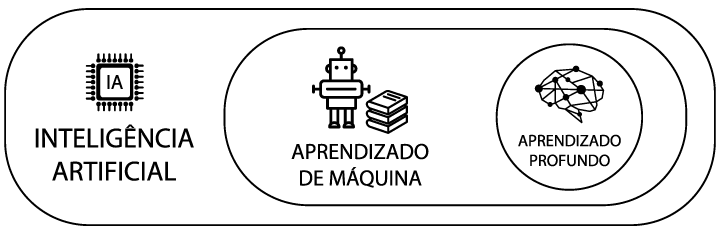
\includegraphics[width=1.0\linewidth]{Imagens/deep.png}
    \caption*{Fonte: Arquivo dos autores (2020)}
    \label{autoai-results}
\end{figure}

\section{Deep Learning e Redes Neurais}

\subsection{História}
\indent
\par O início da história do \textit{deep learning} data de 1943, quando o matemático Walter Pitts e o neurofisiologista Warren McCulloch, baseando-se em pesquisas do cérebro humano, modelaram o primeiro modelo computacional para uma rede neural, baseando-se em neurônios simples, criados a partir de circuitos elétricos. Walter e Warren utilizaram uma combinação de matemática e algoritmos, denominada de lógica de limiar (\textit{threshold logic}), que é utilizada até os dias atuais como base das redes neurais \cite{Academy2019}.

\par Em 1960, Henry J. Kelley desenvolveu o conceito básico de um modelo de retropropagação (\textit{backpropagation}) \cite{Foote2019}, que também é utilizado até os dias atuais para o recálculo dos pesos das redes neurais no processo de aprendizagem. Apesar das descobertas e estudos nas décadas entre 40 a 80, devido à limitação computacional existente na época, o aprimoramento das redes neurais foi severamente impactado até 1981 e o assunto foi subestimado e criticado, além de ter sofrido grande redução no financiamento de pesquisas relacionadas à área.

\par Entretanto, em 1982, John Hopfield apresentou uma abordagem prática para redes neurais, demonstrando como elas poderiam atuar em problemas reais, o que fez com que o assunto voltasse a ter sua devida atenção. Em 1987 ocorreu a primeira Conferência Internacional sobre Redes Neurais do \textit{Institute of Electrical and Electronic Engineer’s} (IEEE). Ao mesmo tempo que o assunto vinha novamente ganhando destaque, o poder computacional da época ainda não conseguia acompanhar o desenvolvimento dos estudos, impossibilitando a criação de grandes aplicações com \textit{deep learning}, o que gerou frustração e novamente uma redução de investimentos na área \cite{Academy2019}.

\par Ainda assim, algumas pessoas continuaram estudando o assunto e em 1995, Dana Cortes e Vladimir Vapnik desenvolveram a máquina de vetores de suporte, um sistema capaz de reconhecer padrões com aprendizado supervisionado \cite{Foote2019}. Nos anos seguintes, a partir de 1999, os computadores começaram a ganhar poder de processamento, viabilizando a implementação de redes neurais mais eficientes, que começaram a competir com as máquinas de vetores de suporte. Apesar de possuírem um maior tempo de processamento, em geral, as redes neurais se mostraram mais assertivas utilizando os mesmos dados e voltaram a ganhar visibilidade no mercado.

\par A partir de então diversos estudos e pesquisas realizados na área e à medida que os computadores foram evoluindo, as aplicações envolvendo redes neurais também o fizeram. Nos anos subsequentes, o algoritmo de aprendizagem profunda do Google foi capaz de identificar gatos em 2012 e em 2014 o Facebook implementou a \textit{DeepFace}, tecnologia capaz de marcar automaticamente os rostos dos usuários da rede social em fotografias. Dois anos depois, o algoritmo do Google \textit{AlphaGo} mapeou o jogo de tabuleiro \textit{Go} e ganhou de Lee Sedol em um torneio em Seul, que à época tinha sido campeão mundial de \textit{Go} 18 vezes \cite{Academy2019}.

\par Com isso, o campo da inteligência artificial e do \textit{deep learning} em especial vem avançando em pesquisas até os dias atuais, além de novamente ter ganhado visibilidade e estar inserido em diversas aplicações corporativas que requerem uma análise de dados mais profunda, com reconhecimento de padrões, previsões ou classificações, por exemplo.

\subsection{Funcionamento das Redes Neurais}

\indent
\par O funcionamento das redes neurais atuais pode ser explicado tendo como base o perceptron elementar, o modelo mais simples e didático de rede neural de camada única.

\begin{figure}[H]
    \centering
    \caption{Perceptron Elementar}
    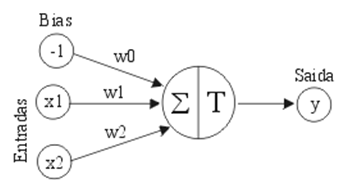
\includegraphics[width=0.6\linewidth]{Imagens/perceptron.png}
    \caption*{Fonte: UFSC, s.d. (\url{https://www.gsigma.ufsc.br/~popov/aulas/rna/neuronio_implementacao/})}
    \label{perceptron}
\end{figure}

\par No modelo apresentado (Figura \ref{perceptron}), constituído por apenas um único neurônio artificial, duas entradas, uma unidade de \textit{bias} e uma saída, cada entrada possui pesos w0, w1 e w2 associados a elas, assim como a unidade de \textit{bias}, que também funciona como uma entrada, mas possui seu valor fixado normalmente em 1 ou -1, com a finalidade de aumentar o grau de liberdade do ajuste dos pesos. Por padrão, em bibliotecas que possibilitam a implementação de redes neurais, a unidade de \textit{bias} já é definida automaticamente.

\par Assim sendo, o algoritmo que simula o neurônio irá multiplicar cada entrada por seu respectivo peso para todas as entradas e realizar a somatória de todos esses resultados. Após a obtenção do valor da somatória, ele deve ser submetido a uma função de ativação ou transferência T, gerando a saída y. Dentre outras funções de transferência, pode-se citar a função sigmoide, tangente hiperbólica, unidade linear retificada (ReLU) e unidade linear exponencial (ELU).

\par Durante os estudos e desenvolvimento de algoritmos para redes neurais, ficou claro que para problemas mais complexos, seria necessário expandir a quantidade de neurônios e de camadas, tornando a saída de um neurônio, a entrada para o próximo. A quantidade de neurônios e de camadas deve ser estudada e testada individualmente para cada problema que se pretende solucionar, variando caso a caso.

\begin{figure}[H]
    \centering
    \caption{Rede Neural Multicamada}
    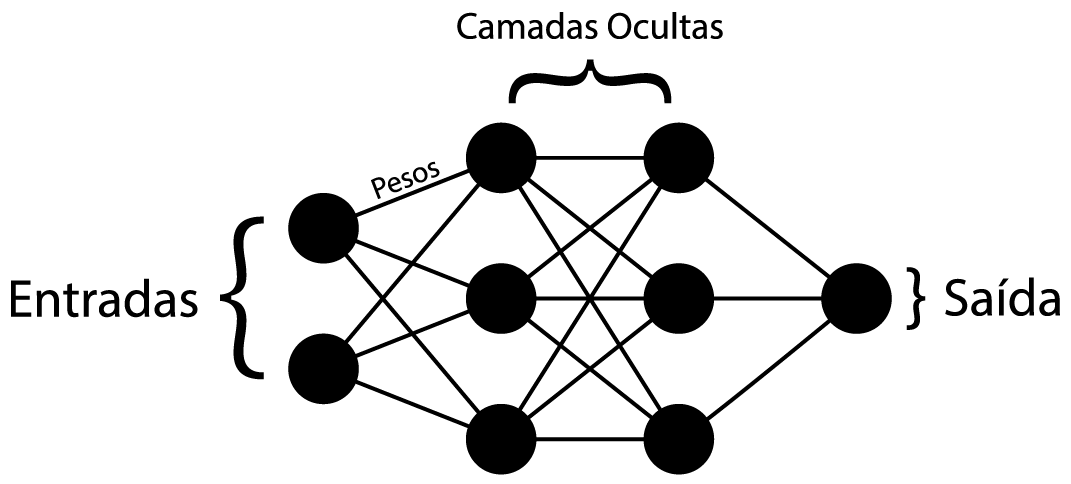
\includegraphics[width=1.0\linewidth]{Imagens/rede-neural.png}
    \caption*{Fonte: Arquivo dos autores (2020)}
    \label{redeneural}
\end{figure}

\par As redes neurais artificiais multicamadas são divididas basicamente em três principais partes: entradas, camadas ocultas e saída, podendo ser uma ou várias dependo do tipo de problema. Nesse tipo de rede, uma série de neurônios são interligados como mostrado e quando uma saída é obtida, ela é comparada com uma saída considerada correta, gerando um valor de erro. Com base nesse erro, os pesos são então recalculados utilizando o conceito de gradiente para a minimização do erro, até que seu valor seja considerado satisfatório. Essa etapa em que os pesos são recalculados e a rede neural está sofrendo alterações é denominada de treinamento.

\par Após essa fase, a rede deve ser testada com dados diferentes dos que foram usados durante o treinamento para garantir sua assertividade. Essa etapa recebe o nome de teste. Caso comprovada sua eficiência e as taxas de erro permanecerem baixas, a rede neural está apta para ser utilizada com dados novos obtidos de um contexto real.



\section{Análise de imagens de câmeras de ônibus}

\indent
\par Com o avanço da tecnologia nos últimos anos, pode-se observar o surgimento de algumas aplicações envolvendo a interpretação de imagens das câmeras em transportes públicos. Em 2014, por exemplo, um grupo da Universidade de Parma, Itália, divulgou um artigo \cite{Bernini2014} sobre um estudo de contagem de passageiros em ônibus utilizando câmeras que seriam instaladas sobre as portas dos veículos e enviaram as imagens para um computador a bordo capaz de processar as imagens e reconhecer a cabeça das pessoas, realizando uma comparação com esferas. Contudo, esse processo ainda necessitava de melhorias devido à similaridade de outros objetos com esferas, resultando em falsos positivos e ao seu tempo de processamento, que levava 100 ms.

\par Em 2019, outra aplicação de análise de imagens no transporte público pode ser citada. Em Bangalore, Índia,  um diretor do BMTC (Bengaluru Metropolitan Transport Corporation), órgão responsável pelos ônibus da cidade, anunciou que iniciaria testes em conjunto com Instituto Indiano de Ciência (IISc) nos quais dados provenientes de câmeras instaladas nos ônibus iriam ser enviados para servidores e certos comportamentos do motorista como velocidade e sono seriam analisados \cite{Prasad2019}.

\par Além disso, em maio de 2020, foi implantado nas câmeras dos ônibus da França um sistema que permite analisar o uso de máscaras e o distanciamento social dentro dos veículos como tentativa de prevenir o contágio em meio a crise de Covid-19 \cite{BBC2020}. A iniciativa partiu da \textit{startup} Datakalab, que garante a privacidade dos passageiros e afirma que o algoritmo não realiza detecção facial, analisando apenas as informações necessárias e avisando as autoridades quando necessário.

\subsection{Detecção de objetos em tempo real com YOLO}

\indent
\par A lotação dos ônibus é um fator determinante para o ajuste correto das frotas de ônibus e dentre outras informações, será um importante indicativo presente no \textit{dashboard} que será desenvolvido neste trabalho. Uma das maneiras de se extrair essa informação é a partir de uma análise baseada em inteligência artificial das imagens de câmeras instaladas dentro dos veículos, disponibilizadas em tempo real.

\par Em comparação com outros detectores de imagem, o YOLO, do inglês \textit{You Only Look Once} (você só olha uma vez), se mostrou uma ferramenta extremamente rápida e com alta acuracidade \cite{RedmonJosephandFarhadi2018}, que utiliza um método que analisa a imagem apenas uma vez para realizar a detecção de objetos, dando origem ao seu nome e garantindo sua rapidez.

\par O funcionamento do YOLO baseia-se em redes neurais convolucionais \cite{RedmonJosephandFarhadi2018}, um tipo específico de rede neural, e inicia-se dividindo a imagem em uma malha S x S contendo um determinado número de células. Em seguida, cada célula torna-se responsável por criar caixas delimitadoras de objetos, assim como prever a probabilidade dessas caixas conterem um objeto em específico. A partir disso, um mapa com diversas caixas delimitadoras é criado para a imagem, contendo a localização de cada objeto detectado. Contudo, muitas destas caixas possuem precisão muito baixa e então apenas as com maior precisão são mantidas. A Figura \ref{funcyolo} representa esse funcionamento.

\begin{figure}[H]
    \centering
    \caption{Etapas da detecção de objetos do YOLO}
    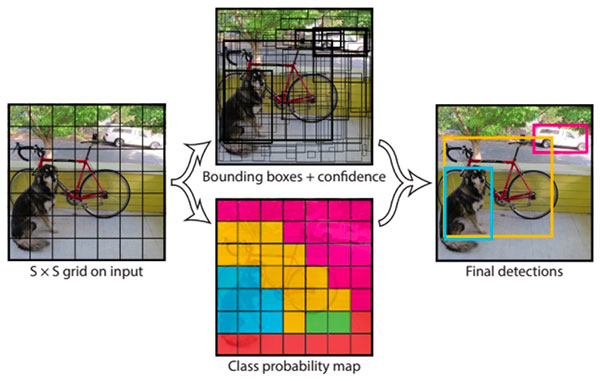
\includegraphics[width=0.6\linewidth]{Imagens/yolo-design.jpg}
    \caption*{Fonte: Rosebrock, Adrian, 2018 (\url{https://www.pyimagesearch.com/2018/11/12/yolo-object-detection-with-opencv/})}
    \label{funcyolo}
\end{figure}

\par Por fim, vale ressaltar que o YOLOv3, versão mais nova da ferramenta disponível atualmente, quando comparado com outras ferramentas de mesma finalidade apresenta em média uma precisão parecida na escala mAP-50 (utilida para medir a precisão dos algoritmos de reconhecimento de imagens), porém sua velocidade de processamento é maior, chegando a ser quatro vezes mais rápido (Figura \ref{speedyolo}). Assim sendo, para análise de imagens em tempo real, nas quais a velocidade é crucial, o YOLO revela-se uma excelente alternativa.

\begin{figure}[H]
    \centering
    \caption{Comparação do YOLO com outras ferramentas}
    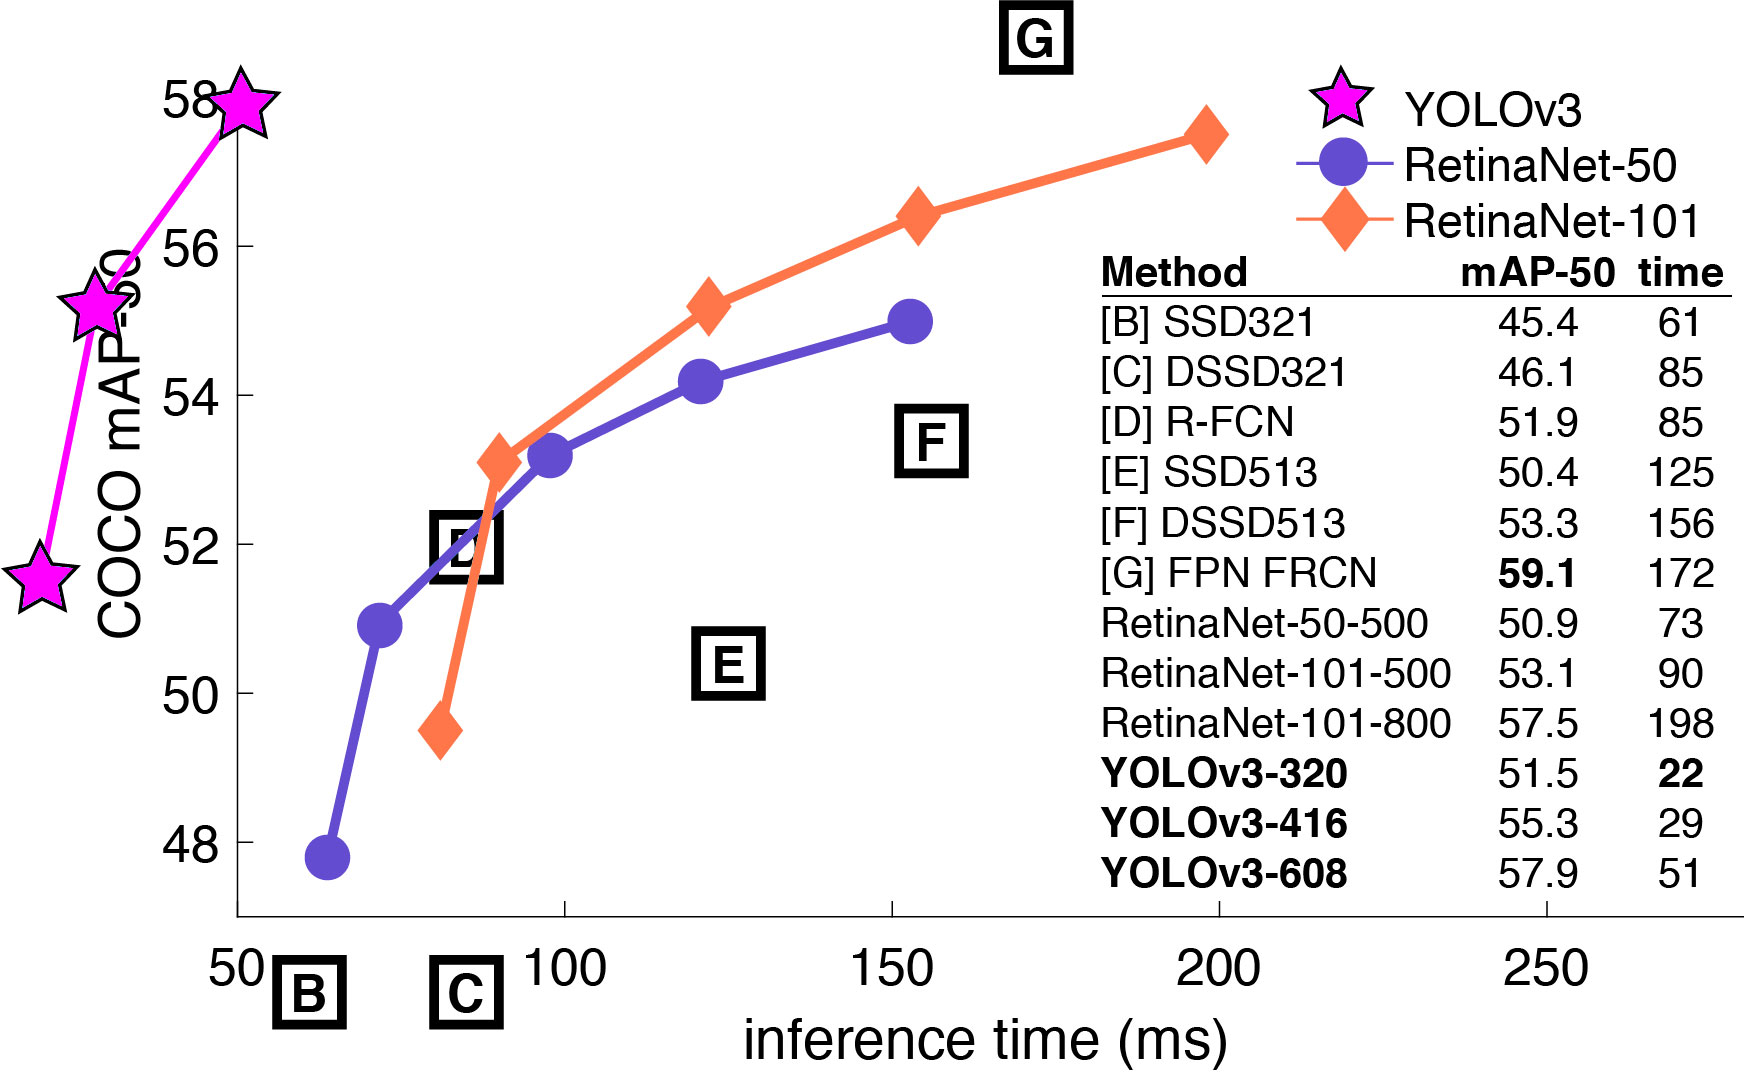
\includegraphics[width=0.6\linewidth]{Imagens/yolo-speed.jpg}
    \caption*{Fonte: Redmon, Joseph e Farhadi, Ali, 2018 (\url{https://pjreddie.com/darknet/yolo/})}
    \label{speedyolo}
\end{figure}

\section{Análise de Dados}

\indent
\par Apesar de estar cada vez mais em destaque nestes últimos anos, podemos traçar o uso de estatística para tomada de decisão desde do Egito Antigo, de acordo com um artigo publicado por Keith D. Foote \cite{Foote2018} os egípcios já usavam cálculos estatísticos para construir as pirâmides. Já na década de 1880, o governo americano levou pelo menos 7 anos para completar o censo da população, processo que foi reduzido para um ano e meio na década seguinte por causa do desenvolvimento de uma máquina de tabulação, por Herman Hollerith, que processava os dados de forma sistêmica em cartões perfurados.

\subsection{Primeira fase da análise de dados}

\indent
\par Trazendo para os dias atuais, a Universidade de Villanova separa a análise de dados em três estágios \cite{Villanova}. O primeiro deles seria o início do que chamamos de \textit{Business Intelligence}, que surgiu por volta de 1950 como uma forma de processar pequenas quantidades de informações estruturadas. Esse estágio, que podemos chamar de \textit{Analytics 1.0}, durou até cerca de 2009, quando foi consolidado o termo \textit{"big-data"}.

\par O fim do primeiro estágio se deu pelo aumento exponencial de dados sendo produzidos diariamente, podendo vir de qualquer lugar e forma, desde de informações simples e estruturadas, como quais produtos alguém comprou em um determinado site, ou coisas mais complexas, como quais sites fizeram essa pessoa chegar até uma determinada página e qual a posição geográfica dessa pessoa quando acessou a página. Se convencionou a chamar esses dados em grande quantidade e pouco estruturados de \textit{"big-data"}.

\subsection{Segunda fase da análise de dados}

\indent
\par Pela dificuldade de armazenar e processar essa massiva quantidade de dados, se fez necessário o desenvolvimento de novos métodos e ferramentas para o processamento deles, o que deu início ao \textit{Analytics 2.0}, que trouxe alternativas como Hadoop, que pode processar essas grandes massas de dados, e o NoSQL, que permite armazenar toda a informação de forma mais eficiente que os bancos de dados relacionais faziam até então. Além disso, cada vez mais se fez necessário um conhecimento tecnológico para fazer essas análises, quando até então bastava o conhecimento de métodos estatísticos.

\subsection{Terceira fase da análise de dados}

\indent
\par Hoje em dia, muitos especialistas dizem que chegamos a um terceiro estágio, o \textit{Analytics 3.0}, onde esses dados que são produzidos a qualquer momento podem ser usados como moeda de troca entre consumidor e fornecedor. Essa moeda pode ser analisada imediatamente pelo fornecedor, que passa a entregar uma experiência personalizada para quem está consumindo o seu produto.

\subsection{Análise de dados no dia a dia}

\indent
\par Com a disponibilidade de dados que temos, as empresas estão se dedicando cada vez mais em coletar e auxiliar as suas decisões nas análises feitas com eles. O Diretor de Estratégia e Marketing de Precisão da Coca-Cola, Justin De Graaf, afirmou em entrevista para ADMA, Association for Data-Driven Marketing \& Advertising, que cada vez mais a empresa usa informações coletadas diretamente dos consumidores, como por meio de telefone, redes sociais ou \textit{e-mail}, para criar desde campanhas publicitárias até novos produtos \cite{Tan2017}. Outra marca consolidada usando análise de dados para a tomada de decisão é a rede de hotéis Marriott, que, de acordo com o seu \textit{chief development officer}, Eric Jacobs, tem usado esse tipo de informação para decidir como identificar, atrair e manter os seus cliente mais lucrativos \cite{Eisen2018}. Para isso eles coletam desde dados como padrão social dos clientes até se eles consomem mais jeans Levi's ou Gap.

\par Apesar disso, alguns resultados dessas análises podem ter um efeito contrário do que era pretendido no início. Caso a análise não seja feita com atenção, verificando sempre quem está sendo atingido, ela pode levar a alguns atritos e desgastar a imagem de quem usa essas informações.

\par Em 2012, o New York Time publicou uma história de como um pai descobriu a gravidez da filha através de uma promoção oferecida pela rede varejista Target, nos Estados Unidos \cite{Duhigg2012}. Andrew Pole, um estatístico da rede, foi designado para desenvolver um "preditor de gravidez", no fim do estudo ele conseguiu chegar a uma lista de 25 produtos, que geram uma probabilidade da cliente estar grávida de acordo com o seu preditor. Esses produtos contêm itens como manteiga de cacau, bolsas grandes o suficiente para caber pacotes de fraldas, e suplementos como magnésio e zinco.

\par A Target vinculava essa informação a um identificador do cliente, e então ofereceria um desconto na próxima visita que essa mesma pessoa fizesse a loja. Um ano após a aplicação deste preditor, o pai de uma adolescente foi a uma das lojas reclamar que sua filha tinha recebido um desconto relacionado a esse programa específico para grávidas, com isso, o gerente da loja se desculpou pelo erro e alguns dias depois ligou para se desculpar novamente. Entretanto, para a surpresa do gerente, durante essa ligação o cliente disse que a filha não tinha contado para ele que estava grávida, e que a Target soube antes dele do acontecido. Após esse caso, o departamento de \textit{marketing} decidiu desacelerar o programa de análises de dados, e passar mais tempo avaliando qual impacto cada iniciativa pode ter.
 \cleardoublepage
		\chapter{Metodologia}
\label{Cap:MateriaisMetodos}

% Capítulo 3: Materiais e Métodos (ou Metodologia)

XXXXX

%revisar introdução acima depois de finalizado o capítulo

\section{Assunto 1}

XXXXXXXX

%\begin{figure}[H]
%    \centering
%    \caption{Diagrama da solução}
%    \includegraphics[width=0.9\linewidth]{Imagens/diagramaSimplificado3.png}
%    \caption*{Fonte: Arquivo dos autores (2019)}
%    \label{diag-solucao}
%\end{figure}

\subsection{SubAssunto 1}

XXXXXX
\\\\
XXXXXX


 \cleardoublepage
		\chapter{Resultados Obtidos}
\label{Cap:Resultados}
\newcommand{\EscalaAlgumaCoisa}{0.6}

% Capítulo 4: Resultados

xxxxx

\\\\
xxxxx 

\section{Figuras}

xxxxx

%\begin{figure}[H]
%    \centering
%    \caption{Resultados da ferramenta AutoAI - IBM}
%    \includegraphics[width=1.0\linewidth]{Imagens/autoai-results.png}
%    \caption*{Fonte: Arquivo dos autores (2019)}
%    \label{autoai-results}
%\end{figure}

\section{Tabelas}

xxxxx

\section{Equações}

xxxxx

\section{Códigos Fonte de Programação}

xxxxx

 \cleardoublepage
		\chapter{Conclusão e Trabalhos futuros}
\label{Cap:Conclusoes}
% Capítulo 5: Conclusões
\indent
\par Considerando o objetivo deste projeto de reunir diversas informações de fontes diferentes, disponibilizá-las de uma forma prática e transparente para toda a população e para gestores da SPTrans como ferramenta de apoio à decisão, pode-se concluir que o \textit{dashboard} desenvolvido atende às demandas citadas. Por meio dele, painéis e gráficos em tempo real exibem informações relevantes do transporte público, que são facilmente acessadas por qualquer cidadão por meio de uma página web.
\indent
\par Além disso, a possibilidade de implementação do sistema em outras empresas de transporte público e privado, juntamente com a diversificação dos dados obtidos e armazenados, aumentam a aplicabilidade do projeto. Vale ainda ressaltar que como próximos passos, a aplicação ainda pode ser continuamente aprimorada com a análise dos dados armazenados, que irão aumentar ao longo do tempo.
\indent
\par Tendo em vista que a aplicação salva dados diariamente, a quantidade de informações armazenadas tende a crescer rapidamente. Com isso, o espaço em disco, memória e CPU necessários na instância EC2 que armazena o banco de dados precisaria aumentar paralelamente aos dados. Por esse motivo, seria válido que o banco de dados ficasse em uma instância apartada da instância de aplicação, garantindo maior escalabilidade e persistência dos dados. Esse objetivo poderia ser alcançado utilizando o serviço RDS da AWS.
\indent
\par Juntamente com a criação de uma nova instância para o banco de dados, considerando que a aplicação já esteja armazenando informações há um longo período, também seria viável um estudo mais aprofundado das informações e a aplicação de técnicas de inteligência artificial, por meio das quais seria possível a extração de informações como a previsão de velocidade e atrasos de uma via, previsão de frota, tempo, trânsito etc. Essas e outras informações poderiam ser obtidas, analisadas e incluídas no painel.
\indent
\par Por fim, outra informação que agregaria valor no projeto seria a lotação dos ônibus, que poderia ser extraída por meio de análise de imagens de câmeras já existentes, instaladas dentro dos veículos. Essas imagens passariam por um tratamento e treinamento em uma rede artificial que seria utilizada pelo yolo, que por sua vez identificaria a quantidade de pessoas presentes dentro de cada veículo, classificando cada ônibus como “vazio”, “normal” ou “cheio”.




 \cleardoublepage

		% Apêndices
		%\begin{apendicesenv}
        	%\partapendices
			%\chapter{\textit{ENDPOINTS}}
 \label{app:apendiceA}
\section{/api/onibus-lotacao/}
\textit{GET}
\begin{lstlisting}
{
    "id": 1,
    "id_onibus": 96587,
    "id_linha": 2215,
    "lotacao": "cheio",
    "latitude": "45.658000000000001",
    "longitude": "12.987000000000000",
    "data_inclusao": "2020-10-09T19:41:53.075905Z"
}    
\end{lstlisting}
\textit{POST}
\begin{lstlisting}
{
    "img": caminho_img,
    "id_onibus": id_onibus,
    "id_linha": id_linha,
    "latitude": latitude,
    "longitude": longitude            
}
\end{lstlisting}
\section{/api/onibus-posicao/}
\textit{GET}
\begin{lstlisting}
{
    "quantidade": 11992
}
\end{lstlisting}
\textit{POST}
\begin{lstlisting}
{
    "o": [
        {
            "id_onibus": id_onibus,
            "onibus_deficiente": onibus_deficiente,
            "horario_atualizacao_localizacao": horario_atualizacao_localizacao,
            "latitude": latitude,
            "longitude": longitude,
            "id_linha": id_linha,
            "frota": frota,
        }
    ]
}
\end{lstlisting}
\section{/api/onibus-velocidade/}
\textit{GET}
\begin{lstlisting}
{
    "id": 1067508,
    "nome": "BUTANTA (BAIRRO - CENTRO)",
    "vel_trecho": 27,
    "vel_via": 27,
    "trecho": "de R. AMARO CAVALHEIRO ate R. PAES LEME",
    "extensao": 650,
    "tempo": "00:01",
    "coordenadas": [
        {
            "latitude": "-23.567653",
            "longitude": "-46.695722",
            "id": 6217
        },
        {
            "latitude": "-23.568001",
            "longitude": "-46.696452",
            "id": 6218
        },
        {
            "latitude": "-23.568063",
            "longitude": "-46.696595",
            "id": 6219
        }
}
\end{lstlisting}
\textit{POST}
\begin{lstlisting}
{
    "o": [
        {
            "name": nome,
            "description": {
                'vel_trecho': vel_trecho,
                'vel_via': vel_via,
                'trecho': trecho,
                'extensao': extensao,
                'tempo': tempo
            },
            "coordinates": {
                'lat': latitude,
                'lon': longitude
            }
        }
    ]
}
\end{lstlisting}
\section{/api/linhas/}
\textit{GET}
\begin{lstlisting}
{
    "id_linha": 264,
    "letreiro": "509J-10",
    "sentido": 1,
    "letreiro_destino": "PQ. IBIRAPUERA",
    "letreiro_origem": "JD. SELMA"
}
\end{lstlisting}
\textit{POST}
\begin{lstlisting}
{
    "l": [
        {
            "id_linha": id_linha,
            "letreiro": letreiro,
            "sentido": sentido,
            "letreiro_destino": letreiro_destino,
            "letreiro_origem": letreiro_origem,
        }
    ]
}    
\end{lstlisting}
\section{/api/paradas/}
\textit{GET}
\begin{lstlisting}
{
    "id": 1,
    "id_parada": 4203724,
    "nome": "",
    "endereco": "R. Agamenon Pereira da Silva",
    "latitude": "-23.692865000000001",
    "longitude": "-46.778350000000003"
}
\end{lstlisting}
\textit{POST}
\begin{lstlisting}
{
    "p": [
        {
            "id_parada": id_parada,
            "nome": nome,
            "endereco": endereco,
            "latitude": latitude,
            "longitude": longitude,
        }
    ]
}
\end{lstlisting}
\section{/api/trens/}
\textit{GET}
\begin{lstlisting}
{
    "id": 1,
    "id_linha": 1,
    "data_ocorrencia": "2020-10-07T07:42:01.039607Z",
    "descricao": null,
    "ultima_atualizacao": "2020-10-07T21:14:01.162598Z",
    "situacao": "Operacao Normal"
}
\end{lstlisting}
\textit{POST}
\begin{lstlisting}
{
    "t": [
        {
            "id_linha": id_linha,
            "data_ocorrencia": data_ocorrencia,
            "descricao": descricao,
            "ultima_atualizacao": ultima_atualizacao,
            "situacao": situacao,
        }
    ]
}
\end{lstlisting}
\section{/api/climatempo/}
\textit{GET}
\begin{lstlisting}
{
    "id_cidade": 3477,
    "temperatura": "27.00",
    "direcao_vento": "S",
    "velocidade_vento": "9.00",
    "umidade": "66.00",
    "condicao": "Nuvens esparsas",
    "pressao": "1015.00",
    "sensacao": "28.00",
    "date": "2020-10-07T21:14:34.451818Z"
}
\end{lstlisting}
\textit{POST}
\begin{lstlisting}
{
    "ct": [
        {
            "id_cidade": id_cidade,
            "temperatura": temperatura,
            "direcao_vento": direcao_vento,
            "velocidade_vento": velocidade_vento,
            "umidade": umidade,
            "condicao": condicao,
            "pressao": pressao,
            "sensacao": sensacao,
        }
    ]
}
\end{lstlisting}
\section{/api/eventos/}
\textit{GET}
\begin{lstlisting}
{
    "id": 26,
    "nome": "Maria Bethania",
    "link": "http://premier.ticketsforfun.com.br/shows/show.aspx?sh=MARIBUB19",
    "data_info": "Sao Paulo no UnimedHall 27 de junho",
    "data": "2020-06-27",
    "endereco": "Av. das Nacoes Unidas, 17955 - Vila Almeida, Sao Paulo - SP, 04795-100, Brazil",
    "latitude": "-23.647672600000000",
    "longitude": "-46.723812100000004",
    "data_inclusao": "2020-10-14T00:17:58.612131Z"
}
\end{lstlisting}
\textit{POST}
\begin{lstlisting}
{
    "e": [
        {
            "nome": nome,
            "link": link,
            "data_info": data_info,
            "data": data,
            "endereco": endereco,
            "latitude": latitude,
            "longitude": longitude
        }
    ]
}
\end{lstlisting}
 


%			\include{apendicec}
		%\end{apendicesenv}

		% Anexos
		%\begin{anexosenv}
			%\partanexos % Imprime uma página indicando o início dos anexos
		%\end{anexosenv}
\nocite{}
\bibliography{referencias}
\end{document}
